\subsection*{(5)}
\subsubsection*{解説}
固有エネルギー$\varepsilon$が$E$以下となる状態数$\Omega_3(E)$は
\begin{align}
  \varepsilon=\left(n_x+n_y+n_z+\frac{3}{2}\right)\hbar\omega&\leq E\\
  n_x+n_y+n_z&\leq \frac{E}{\hbar\omega}-\frac{3}{2}
\end{align}
ここで$n$を
\begin{align}
  n&=\frac{E}{\hbar\omega}-\frac{3}{2}\\
  E&=(n+\frac{3}{2})\hbar\omega
\end{align}
とする.ここで$n_x+n_y+n_z=n$を満たすのは図\ref{fig:last}の格子点である.
したがってその数は
\begin{align*}
  \sum_{m=0}^{n}(m+1)=\frac{(n+1)(n+2)}{2}
\end{align*}
となる.したがって状態数$\Omega_3(E)$は
\begin{align}
  \Omega_3(E)&=\frac{(n+1)(n+2)}{2}\\
  &=\frac{1}{2}\left(\left(\frac{E}{\hbar\omega}\right)^2-\frac{1}{4}\right)
\end{align}
となり,状態密度$D_3(E)$は
\begin{align}
  D_3(E)&=\frac{{\rm d}}{{\rm d}E}\Omega_3(E)\\
  &=\frac{E}{\hbar^2\omega^2}
\end{align}

\begin{figure}[hptb]
  \begin{center}
    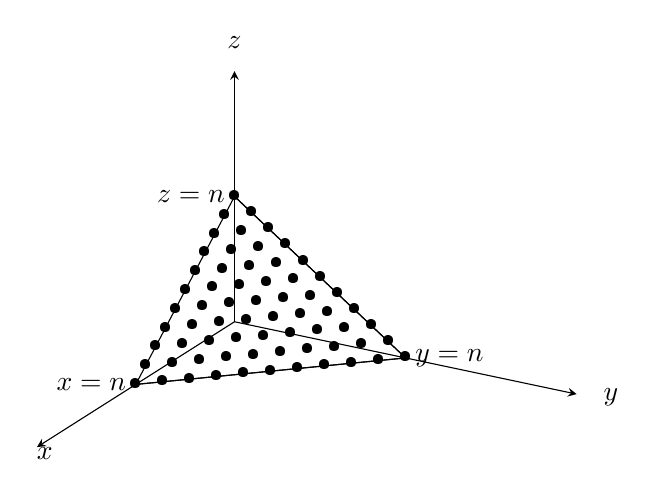
\begin{tikzpicture}[scale=1]
      \begin{axis}[
        view={120}{30},
        axis lines=center,
        ticks=none,
        xmin=0, xmax=20, ymin=0, ymax=20, zmin=0, zmax=20,
        xlabel=$x$, ylabel=$y$, zlabel=$z$,
        every axis x label/.style={
          at={(ticklabel* cs:1.05)},
          anchor=west,
          },
          every axis y label/.style={
            at={(ticklabel* cs:1.05)},
            anchor=west,
            },
            every axis z label/.style={
              at={(ticklabel* cs:1.05)},
              anchor=south,
              }
              ]
              %
              %\node at(axis cs:20,20,20) [anchor=west]{$\boldsymbol{n}$};
              %\draw[-stealth,red,very thick] (axis cs:10,10,10) -- (axis cs:20,20,20);
              \node at(axis cs:10,0,0) [anchor=east]{$x=n$};
              \node at(axis cs:0,10,0) [anchor=west]{$y=n$};
              \node at(axis cs:0,0,10) [anchor=east]{$z=n$};
              \draw[thin] (axis cs:10,0,0) -- (axis cs:0,10,0);
              \draw[thin] (axis cs:10,0,0) -- (axis cs:0,0,10);
              \draw[thin] (axis cs:0,10,0) -- (axis cs:0,0,10);
              \draw[thin] (axis cs:10,0,0) -- (axis cs:0,10,0) -- (axis cs:0,0,10);
              
              \node at (axis cs:10,0,0) {\textbullet};
              \node at (axis cs:9,1,0) {\textbullet};
              \node at (axis cs:8,2,0) {\textbullet};
              \node at (axis cs:7,3,0) {\textbullet};
              \node at (axis cs:6,4,0) {\textbullet};
              \node at (axis cs:5,5,0) {\textbullet};
              \node at (axis cs:4,6,0) {\textbullet};
              \node at (axis cs:3,7,0) {\textbullet};
              \node at (axis cs:2,8,0) {\textbullet};
              \node at (axis cs:1,9,0) {\textbullet};
              \node at (axis cs:0,10,0) {\textbullet};
              \node at (axis cs:9,0,1) {\textbullet};
              \node at (axis cs:8,1,1) {\textbullet};
              \node at (axis cs:7,2,1) {\textbullet};
              \node at (axis cs:6,3,1) {\textbullet};
              \node at (axis cs:5,4,1) {\textbullet};
              \node at (axis cs:4,5,1) {\textbullet};
              \node at (axis cs:3,6,1) {\textbullet};
              \node at (axis cs:2,7,1) {\textbullet};
              \node at (axis cs:1,8,1) {\textbullet};
              \node at (axis cs:0,9,1) {\textbullet};
              \node at (axis cs:8,0,2) {\textbullet};
              \node at (axis cs:7,1,2) {\textbullet};
              \node at (axis cs:6,2,2) {\textbullet};
              \node at (axis cs:5,3,2) {\textbullet};
              \node at (axis cs:4,4,2) {\textbullet};
              \node at (axis cs:3,5,2) {\textbullet};
              \node at (axis cs:2,6,2) {\textbullet};
              \node at (axis cs:1,7,2) {\textbullet};
              \node at (axis cs:0,8,2) {\textbullet};
              \node at (axis cs:7,0,3) {\textbullet};
              \node at (axis cs:6,1,3) {\textbullet};
              \node at (axis cs:5,2,3) {\textbullet};
              \node at (axis cs:4,3,3) {\textbullet};
              \node at (axis cs:3,4,3) {\textbullet};
              \node at (axis cs:2,5,3) {\textbullet};
              \node at (axis cs:1,6,3) {\textbullet};
              \node at (axis cs:0,7,3) {\textbullet};
              \node at (axis cs:6,0,4) {\textbullet};
              \node at (axis cs:5,1,4) {\textbullet};
              \node at (axis cs:4,2,4) {\textbullet};
              \node at (axis cs:3,3,4) {\textbullet};
              \node at (axis cs:2,4,4) {\textbullet};
              \node at (axis cs:1,5,4) {\textbullet};
              \node at (axis cs:0,6,4) {\textbullet};
              \node at (axis cs:5,0,5) {\textbullet};
              \node at (axis cs:4,1,5) {\textbullet};
              \node at (axis cs:3,2,5) {\textbullet};
              \node at (axis cs:2,3,5) {\textbullet};
              \node at (axis cs:1,4,5) {\textbullet};
              \node at (axis cs:0,5,5) {\textbullet};
              \node at (axis cs:4,0,6) {\textbullet};
              \node at (axis cs:3,1,6) {\textbullet};
              \node at (axis cs:2,2,6) {\textbullet};
              \node at (axis cs:1,3,6) {\textbullet};
              \node at (axis cs:0,4,6) {\textbullet};
              \node at (axis cs:3,0,7) {\textbullet};
              \node at (axis cs:2,1,7) {\textbullet};
              \node at (axis cs:1,2,7) {\textbullet};
              \node at (axis cs:0,3,7) {\textbullet};
              \node at (axis cs:2,0,8) {\textbullet};
              \node at (axis cs:1,1,8) {\textbullet};
              \node at (axis cs:0,2,8) {\textbullet};
              \node at (axis cs:1,0,9) {\textbullet};
              \node at (axis cs:0,1,9) {\textbullet};
              \node at (axis cs:0,0,10) {\textbullet};
              
            \end{axis}
          \end{tikzpicture}
        \end{center}
        \caption{$n_x+n_y+n_z=n$を満たす格子点}
        \label{fig:last}
      \end{figure}